\section{Thread 线程}
\subsection{线程概念}

进程是程序的一次执行过程,是系统运行程序的基本单位,因此进程是动态的。系统运行一个程序即是一个进程从创建,运行到消亡的过程。

线程是进程中的一个实体,线程本身是不会独立存在的。同类的多个线程共享进程的堆和方法区资源,但每个线程有自己的程序计数器、虚拟机栈和本地方法栈,所以系统在产生一个线程,或是在各个线程之间作切换工作时,负担要比进程小得多,也正因为如此,线程也被称为轻量级进程。

线程是 CPU 的基本执行单位,CPU 执行线程一般使用的是时间片轮转法,在单位时间片中,线程可能不会被执行完,程序计数器记录了线程执行的位置,用于下一次执行。每个线程都有自己的局部资源,这些资源被保存在线程私有的栈中。

一个线程的生命周期如下\footnote{图片作者:\url{https://mp.weixin.qq.com/s/UOrXql_LhOD8dhTq_EPI0w}}:

\begin{center}
    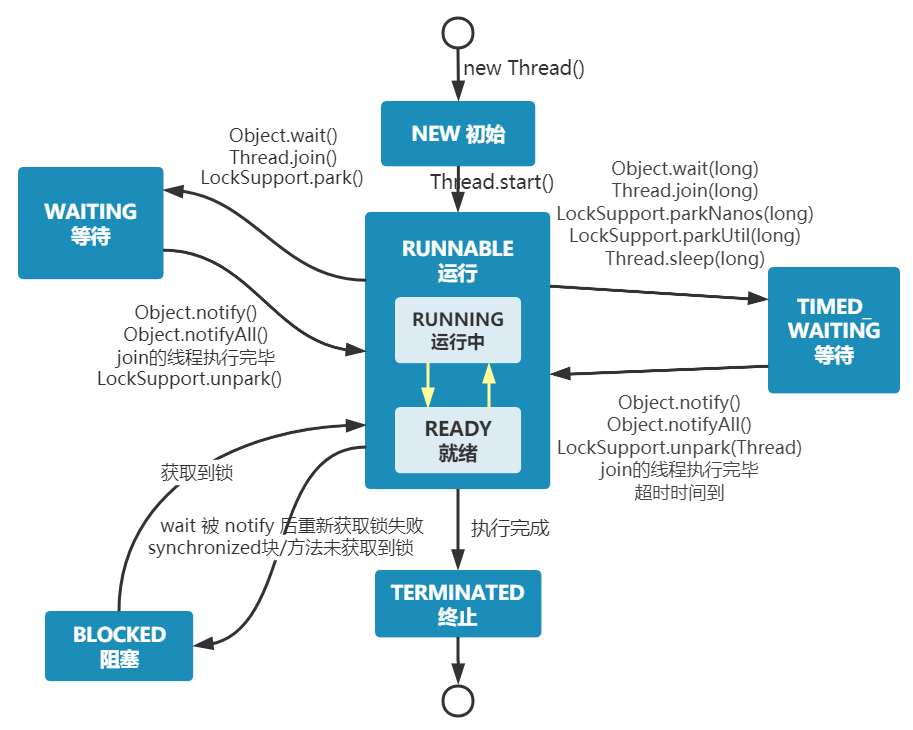
\includegraphics[width=0.8\linewidth]{../../../Images/ThreadProcess.png}
\end{center}

理解线程周期之前,有一些必要的线程属性(均为私有的)需要知道:
\begin{itemize}
    \item volatile String name: 线程名。
    \item int priority: 线程优先级。
    \begin{itemize}
        \item public static final int MAX\_PRIORITY = 10;
        \item public static final int NORM\_PRIORITY = 5;
        \item public static final int MIN\_PRIORITY = 1;
    \end{itemize}
    \item boolean daemon = false: 是否为后台进程。
    \item volatile boolean interrupted: 是否处于终端状态。
    \item Runnable target: 运行目标。
    \item ThreadGroup group: 该线程所属的线程组。
    \item final long stackSize: 该线程所需要的栈大小。
    \item final long tid: 线程 id。
    \item volatile int threadStatus: 线程状态。
    \item volatile Interruptible blocker: 导致线程阻塞的对象。
\end{itemize}

此外,还有几个常用的静态方法(都是公有的):

\begin{itemize}
    \item native Thread currentThread(): 获取当前正在执行的线程。
    \item native void yield(): 使当前线程从 running 变为 ready。可以理解为让步,但也可能下一个执行的还是自己。
    \item native void sleep(long millis): 让当前线程休眠。
    \begin{itemize}
        \item 有时候,我们会使用 sleep(0), 看似没用,但这可以让线程放弃 CPU,释放时间片,让其他线程执行,相当于一个让位动作。
    \end{itemize}
    \item void onSpinWait() {}: 线程让步。
    \begin{itemize}
        \item 这是一个空方法,但是被 @IntrinsicCandidate 注解,意味着在 JVM 中有高效实现,它的主要作用是代替 sleep(0), 因为性能更好。
    \end{itemize}
    \item boolean interrupted(): 判断并重置当前线程的中断状态。
    \item int activeCount(): 获取当前线程组的激活状态的线程数。
    \item int enumerate(Thread tarray[]): 将该线程组及其子组复制到指定数组。
    \item void dumpStack(): 打印当前线程的执行栈。
    \item native boolean holdsLock(Object obj): 判断当前线程持有某个对象的锁。
    \item public static Map<Thread, StackTraceElement[]> getAllStackTraces(): 加强版 dumpStack()。
\end{itemize}

\subsection{线程的构造方法,创建与运行}

这一节说明如何创建 Thread,介绍 Thread 的 start() 方法,这章只涉及 NEW 状态与 RUNNING 状态:

\begin{Java}
public class Thread implements Runnable
\end{Java}

在创建线程之前,先看一下 Thread 的 start() 方法,只有了解了 start() 方法需要什么,才能更好的理解线程的创建与构造函数:

\begin{Java}
public synchronized void start() {
    // 线程状态不为0(not yet started)
    if (threadStatus != 0)
        throw new IllegalThreadStateException();
    // 加入线程组
    group.add(this);
    boolean started = false;
    try {
        // JVM 调用 run 方法
        start0();
        started = true;
    } finally {
        try {
            // 未成功 start,状态记入 group
            if (!started) {
                group.threadStartFailed(this);
            }
        } catch (Throwable ignore) {
            // 不处理 start0 的错误
        }
    }
}
\end{Java}

可以看到,start() 方法只干了两件事:
\begin{itemize}
    \item 调用 native 方法 start0(),核心是调用 run() 方法。
    \item 在线程组 group 中记录该线程的状态。
\end{itemize}

线程组 group 可以自动分配,那么 start() 的核心就是调用 run() 方法:

\begin{Java}
@Override
public void run() {
    if (target != null) {
        target.run();
    }
}
\end{Java}

从 run() 方法源码中可以发现,它是调用的 target 的 run() 方法。那么我们想要启用一个线程就有了两总思路:

\begin{itemize}
    \item 派生出一个 Thread 子类,重写 run() 方法。这样 start() 调用的就是 Thread 子类本身的 run() 方法。
    \item 传入一个 target 对象,调用 target 的 run() 方法。
\end{itemize}

第一种方法不做解释,继承后直接调用 start() 方法即可。第二种方法则需要在 Thread 的构造方法中传入一个 Runnable 对象,由于 Runnable 是函数式接口,因此也可以使用 lambda 表达式快速传入:

\begin{Java}
Thread thread = new Thread(() -> {
    System.out.println(Thread.currentThread().getName());
});
thread.run();
\end{Java}

这两种方法各有好处,具体用哪种视情况而定。

下面看一下 Thread 的构造函数,本质上每个构造函数都调用了 private Thread 方法:

\begin{Java}
private Thread(ThreadGroup g, Runnable target, String name, long stackSize, AccessControlContext acc, boolean inheritThreadLocals)
\end{Java}

在我们实际调用构造函数时,每一个参数都是可选的(因为存在空的构造函数):
\begin{itemize}
    \item g: 默认情况下,由父线程组管理,最顶层的线程组为 main 线程组。
    \item target: 指定的目标对象,调用其 run() 方法,如果没有且没有重写 start() 方法,啥都不干也不抛错。
    \item name: 线程名,不起的话,钩爪函数会自动帮我们起 "Thread-"+nextThreadNum()。
    \item stackSize: 默认构造时为 0。
    \item acc: 如果为 null,会通过 AccessController.getContext() 获取。
    \item inheritThreadLocals: 默认为 true。用于获取一些初始化变量。
\end{itemize}

一般的,我们都是通过构造函数 Thread(Runnable target) 初始化一个线程,再通过 start() 方法让线程进入运行状态。
\begin{itemize}
    \item 初始状态(NEW): 调用构造函数,构造函数会给线程加载各种属性值。
    \item 运行状态(RUNNABLE): 除了 CPU 资源,其余所有资源都具备,线程可以运行。
    \begin{itemize}
        \item 运行中(RUNNING): 线程获取 CPU 时间片,进入运行状态。
        \item 就绪(READY): 线程为获取时间篇,随时准备获取时间片并运行。
    \end{itemize}
\end{itemize}

\subsection{线程通知与等待}

这章介绍 wait() 与 notify() 方法,涉及到 RUNNABLE, BLOCKED, WAITING 状态的转换。

\subsubsection{wait 系列方法}

先看一下 Object.wait() 方法:

\begin{Java}
public final void wait() throws InterruptedException
\end{Java}

无参的 wait() 方法会调用被 native 修饰的其他同名方法,被 interrupt 方法调用时抛出 InterruptedException 错误并清除中断状态。

当一个线程调用一个共享变量的 wait() 方法时,该线程会进入等待(WAITING)\footnote{也也常被称为挂起状态,但挂起是进程的状态,一般认为挂机是进入 WAITING 或 TIMED\_WAITING 状态。}状态,直到发生如下事件:
\begin{itemize}
    \item 其他线程调用了该共享对象的 notify() 或 notifyAll() 方法;
    \item 其他线程调用了该线程的 interrupt() 方法,该线程抛出InterruptedException异常返回。
\end{itemize} 

值得注意的是,即使没有使用如上操作,也没有进行其他手动操作,线程也可能被唤醒(虚假唤醒),虽然虚假唤醒在应用实践中很少发生,但要防患于未然,做法就是不停地去测试该线程被唤醒的条件是否满足。

\begin{Java}
synchronized (obj) {
    while(条件) {
        obj.wait();
    }
}
\end{Java}


另外需要注意的是,如果调用wait()方法的线程没有事先获取该对象的监视器锁,则调用wait()方法时调用线程会抛出IllegalMonitorStateException异常。获取共享变量监视器锁的方式如下\footnote{synchronized 会在下问讲解,这里只知道就行了。}:
\begin{itemize}
    \item 执行 synchronized 同步代码块时,使用该共享变量作为参数。
    \item 调用该共享变量的方法,并且该方法使用了 synchronized 修饰。
\end{itemize}

可以认为 synchronized 关键字代表了监视器锁。只有通过 synchronized 获取了监视器锁,才能调用 wait() 方法。

看这样一段代码:
\begin{Java}
// 生产者线程
synchronized (queue) {
    while(queue.size() == MAX_SIZE) {
        try {
            queue.wait();
        } catch (Exception ex) {
            ex.printStackTrace();
        }
    }
    queue.add(1);
    queue.notifyAll();
}

// 消费者线程
synchronized (queue) {
    while(queue.size() == 0) {
        try {
            queue.wait();
        } catch (Exception ex) {
            ex.printStackTrace();
        }
    }
    queue.poll();
    queue.notifyAll();
}
\end{Java}

当某个线程尝试执行任意一端代码时,会执行如下流程:

\begin{center}
    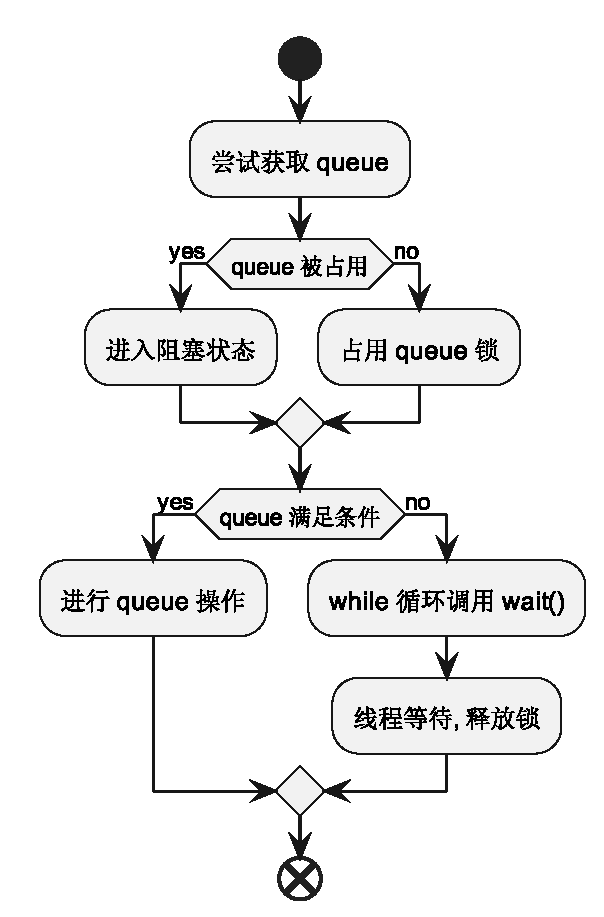
\includegraphics[width=0.4\linewidth]{../../../Images/syn.eps}
\end{center}

当线程调用共享变量的 wait() 方法后,只会释放当前共享变量的锁。此时程序计数器指向获取锁这一步骤,之前的锁并不会被释放,否则程序计数器需要指向其他地方。

wait() 还有两个同名方法,增加了两个参数:
\begin{itemize}
    \item \textbf{wait(long timeoutMillis)}: 这是个 native 方法,wait() 本质上时调用 wait(0),表示不限制时间。 如果一个线程调用共享对象的该方法挂起后,没有在指定的 timeoutMillis 时间内被其他线程调用该共享变量的notify()或者notifyAll()方法唤醒,那么该函数还是会因为超时而返回。
    \item \textbf{wait(long timeoutMillis, int nanos)}: 本质上还是调用 wait(long) 方法,当 nanos 在 (0, Long.MAX\_VALUE) 区间内时,timeoutMillis 自增1。
\end{itemize}

至此我们知道线程不进入 RUNNABLE 态有两种方式:
\begin{itemize}
    \item 获取 synchronized 锁失败,进入阻塞态。
    \item 线程调用资源的 wait 系方法,进入等待态。
\end{itemize}

当线程因为 wait 系方法进入等待态后,对应的资源会维护一个等待队列,将这些线程放入到等待队列中,这个过程在虚拟机中进行。

\subsubsection{notifyAll 系列方法}

首先看一下 notify() 方法,当某个线程调用共享资源的 notify() 方法后,会唤醒一个在该共享资源上调用 wait 系方法后被挂起的资源。一个共享资源上可能有多个线程在等待,具体唤醒哪个线程时随机的。

被唤醒的资源并不能马上从 wait 方法返回并执行,还需要和其他线程一起竞争共享资源锁,然后才能继续执行。notify() 方法同样需要获取共享变量的监视器锁,否则会抛异常。

不同于 notify() 方法只会唤醒一个线程,notifyAll() 方法会唤醒所有在该共享变量上由于调用 wait 系方法而被挂起的线程。

需要注意的是,notify 系方法只会唤醒调用他之前因为 wait 系方法进入等待状态的线程。这在逻辑上很好理解,但在实际运行过程中,我们不知道线程的执行顺序,也就无法判断 notify 方法之前,究竟哪些线程调用了 wait 方法,而在这之后,又会有哪些线程调用 wait 方法。比较常用的方法是通过 Thread.sleep(1000) 让主线程(也可以是其他线程)休眠一定时间,保证其他线程执行完。

我们知道,notify 方法只会唤醒 wait 等待线程,且该线程不会直接获取锁,那么这个过程发生了什么呢:

\begin{itemize}
    \item 同步队列: 尝试获取 Monitor(监视器锁) 失败的线程进入。
    \item 等待队列: 因为 wait 方法等待的线程进入的队列。
\end{itemize}

不同的 notify 方法会唤醒不同的队列元素:
\begin{itemize}
    \item notify: 唤醒等待队列队首的一个线程。
    \item notifyAll: 唤醒等待队列里所有的线程。
\end{itemize}

线程被唤醒后不会直接获取锁并运行,而是进入同步队列队尾,等待获取锁资源。同时我们也知道 Java 常用的队列就有两种: FIFO 的常规队列与优先队列。队列如何实现,后文细说。

\subsubsection{join 线程间等待}

前文所讲的都是线程与共享资源之间的关系,线程之间也存在依赖关系,某个线程的执行需要其他线程执行完,否则需要等待所依赖的线程先执行。

实现这一逻辑的是 Thread 的 join 系方法,该方法和 Object 的 wait 系方法类似,都有三个同名方法,一个无参方法,一个实际起作用的方法。看下核心方法:

\begin{Java}
public final synchronized void join(final long millis) throws InterruptedException {
    if (millis > 0) {
        if (isAlive()) {
            final long startTime = System.nanoTime();
            long delay = millis;
            do {
                wait(delay);
            } while (isAlive() && (delay = millis - TimeUnit.NANOSECONDS.toMillis(System.nanoTime() - startTime)) > 0);
        }
    } else if (millis == 0) {
        while (isAlive()) {
            wait(0);
        }
    } else {
        throw new IllegalArgumentException("timeout value is negative");
    }
}
\end{Java}

所以实际上还是调用了 Thread 本身的 wait 方法,即共享资源是线程本身,由于方法带了 synchronized 关键字,锁了线程对象本身,该方法无需再放入到 synchronized 语句中。

\begin{Java}
Thread threadA = new Thread(() -> {
    ...
    threadB.join(); // 等待 B 线程运行完才能继续运行
    ...
});
\end{Java}

既然 join 系方法本质上是调用 wait 系方法,那么如何唤醒等待线程呢,很遗憾,整个 Thread 类源码里都没有 notify 系方法,那就只能是通过 jvm 唤醒了,查资料可知: 某个线程执行完被关闭之前,jvm 会唤醒所有阻塞在该线程上的其他线程。

\subsection{线程睡眠与让权}

Thread 有一个静态的 sleep 系方法,核心方法被 native 修饰。当某个线程调用该方法时,线程会暂时让出执行权,不参与 CPU 调度。但此时线程不会释放所拥有的监视器资源。指定时间(必须有一个时间参数)后,线程再次进入 READY 状态参与 CPU 调度。在睡眠时同样能被 interrupt 中断。调用该方法,线程将进入 TIMED\_WAITING 状态。

Thread 有一个静态的被 native 修饰的 yield 方法,其作用是暗示线程调度器当前线程请求让出自己的 CPU 使用,但是线程调度器可以无条件忽略这个暗示。

当一个线程调用了Thread类的静态方法yield时,是在告诉线程调度器自己占有的时间片中还没有使用完的部分自己不想使用了,这暗示线程调度器现在就可以进行下一轮的线程调度。

当一个线程调用yield方法时,当前线程会让出CPU使用权,然后处于就绪状态,线程调度器会从线程就绪队列里面获取一个线程优先级最高的线程,当然也有可能会调度到刚让出的线程。

yield 与 sleep 方法的却别在于,yield 只会释放 CPU 资源,不会进入等待状态。yield 方法很少用,造轮子的时候可能会用。

\subsection{线程中断}

Java中的线程中断是一种线程间的协作模式,通过设置线程的中断标志并不能直接终止该线程的执行,而是被中断的线程根据中断状态自行处理。interrupt 系共有三个方法:

\begin{itemize}
    \item \textbf{boolean isInterrupted()}: 判断并清除线程的中断状态。
\begin{Java}
private volatile boolean interrupted;

public boolean isInterrupted() {
    return interrupted;
}
\end{Java}
    \item \textbf{static boolean interrupted()}: 判断当前线程中断状态。
    
如果未被中断,则直接返回中断状态 false,否则清除中断标志,仍然返回 false。

\begin{Java}
public static boolean interrupted() {
    Thread t = currentThread();
    boolean interrupted = t.interrupted;
    if (interrupted) {
        t.interrupted = false;
        clearInterruptEvent();  // native 方法
    }
    return interrupted;
}
\end{Java}
    \item \textbf{void interrupt()}: 中断线程。
    
如果某个线程因为 wait, join, sleep 方法而处于阻塞/等待状态,此时调用其 interrupt() 方法会抛出 InterruptedException 异常。

\begin{Java}
public void interrupt() {
    if (this != Thread.currentThread()) {
        checkAccess();  // 线程可能不让访问
        synchronized (blockerLock) {
            Interruptible b = blocker;
            if (b != null) {
                interrupted = true;
                interrupt0();  // native 方法,通知 jvm 中断线程
                b.interrupt(this);
                return;
            }
        }
    }
    interrupted = true;
    interrupt0();
}
\end{Java}    
\end{itemize}

这些方法的具体实现都依靠虚拟机。

所以 interrupt 方法有什么用呢。如果某个线程等待很长一段时间,为了让其他资源准备完成,但是其他资源可能并不需要这么长的时间,这个时候就可以使用 interrupt 打断正在 sleep 的线程,在 catch 语句中执行接下来要做的事。

\begin{Java}
Thread threadA = new Thread(()->{
    try {
        System.out.println("begin sleep for 200s");
        Thread.sleep(200*1000);
        System.out.println("threadA awake");
    } catch (InterruptedException e) {
        System.out.println("threadA is interrupted while sleeping");
        return;
    }
    System.out.println("threadA leaving normally");
});

threadA.start();
Thread.sleep(1000); // 确保线程A进入睡眠状态
threadA.interrupt();
threadA.join();
System.out.println("main thread over");
\end{Java}

运行结果如下:

\begin{Java}
begin sleep for 200s
threadA is interrupted while sleeping
main thread over
\end{Java}

\subsection{线程知识点补充}

\subsubsection*{线程死锁}

线程上下文切换: 当前线程使用完时间片后,就会处于就绪状态并让出CPU让其他线程占用。线程上下文切换时机有:
\begin{itemize}
    \item 当前线程的CPU时间片使用完转变为就绪状态
    \item 当前线程被其他线程中断
\end{itemize}

线程死锁: 两个或两个以上的线程在执行过程中,因争夺资源而造成的互相等待的现象,在无外力作用的情况下,这些线程会一直相互等待而无法继续运行下去。

如果已经造成了死锁,只有两种方案可以解开: 请求并持,环路等待。在实际运用中,最好的方案是所有使用共享资源的线程都按顺序竞争共享资源,这样就一定不会造成死锁。但是项目越复杂,这就越难做到。

\subsubsection*{守护线程与用户线程}

Java 中的线程分为两类: daemon 线程(守护线程)和 user 线程(用户线程)。默认情况下,我们创建的线程都是用户线程,这两者的区别如下:
\begin{itemize}
    \item 守护线程: JVM 内部启动的线程,比如 GC 线程。
    \item 用户线程: 我们创建的线程,只要存在用户线程未执行结束,JVM 就不会退出。
\end{itemize}

我们可以通过 setDaemon(boolean) 方法设置线程类型。

另外,主线程结束子线程并不一定会结束,有时候即使 main 线程结束,其他用户线程仍在运行,jvm 就不会退出。

\subsection{ThreadLocal}

\subsubsection{ThreadLocal 使用}

多线程访问同一个共享变量时特别容易出现并发问题,特别是在多个线程需要对一个共享变量进行写入时(读变量一般不会出问题)。为了保证线程安全,一般使用者在访问共享变量时需要进行适当的同步,同步的措施一般是加锁,但这需要使用者对锁有一定的了解。

ThreadLocal 可以做到这样的事: 当创建一个变量后,每个线程对其进行访问的时候访问的是自己线程的变量。虽然 ThreadLocal 并不是为了干这样的事而被设计出来的。

创建一个ThreadLocal变量后,每个线程都会复制一个变量到自己的本地内存。

\begin{Java}
static ThreadLocal<String> threadLocal = new ThreadLocal<>();
public static void main(String[] args) throws InterruptedException {
    Thread threadA = new Thread(() -> {
        threadLocal.set("My name is thread A");
        System.out.println(threadLocal.get());
    });
}
\end{Java}

查看 ThreadLocal 源码可知,它一共有一个构造函数,三个公有实例方法,一个静态函数:

\begin{itemize}
    \item void ThreadLocal(): 无参构造函数,什么都不做。
    \item void set(): 设置当前线程的变量。
    \item T get(): 获取当前线程的变量。
    \item void remove(): 移除当前线程的变量。
    \item static <S> ThreadLocal<S> withInitial(Supplier<? extends S> supplier): 构建 ThreadLocal 对象的静态方法。
\end{itemize}

第一次使用 ThreadLocal 会非常令人费解,它的作用是为线程维护``私有''变量,但是为什么这些变量全放在一个 ThreadLocal 对象里呢? 下面看一下 set() 源码:

\begin{Java}
public void set(T value) {
    Thread t = Thread.currentThread();
    ThreadLocalMap map = getMap(t);
    if (map != null) {
        map.set(this, value);
    } else {
        createMap(t, value);
    }
}
\end{Java}

这里只能看出 ThreadLocal 是通过 ThreadLocalMap(一个定制化 HashMap) 维护线程``私有''变量,这个 map 在哪,还需要继续看 getMap 源码:

\begin{Java}
// ThreadLocal
ThreadLocalMap getMap(Thread t) {
    return t.threadLocals;
}
void createMap(Thread t, T firstValue) {
    t.threadLocals = new ThreadLocalMap(this, firstValue);
}
public void remove() {
    ThreadLocalMap m = getMap(Thread.currentThread());
    if (m != null) {
        m.remove(this);
    }
}
// Thread
ThreadLocal.ThreadLocalMap threadLocals = null;
\end{Java}

这下明了了,Thread 对象本身会持有一个 ThreadLocal.ThreadLocalMap 对象,用于保存线程``私有''变量,而这个线程私有变量具体的存取操作则由 ThreadLocal 对象完成,Thread 本身没有对 ThreadLocalMap 的功能性操作,也即在设计本地变量时将对本地变量的操作抽离到了 ThreadLocal 对象上,ThreadLocal 本质是一个工具类。

另外,值得注意的是,一个 threadLocal 只能存储一个本地变量。threadLocal 会提供一个哈希值和本地变量一起作为键值对被存在 Thread 的 ThreadLocalMap 中。

ThreadLocal 中还有一个静态方法,用于快速构建本地变量(不需要再set):

\begin{Java}
public static <S> ThreadLocal<S> withInitial(Supplier<? extends S> supplier) {
    return new SuppliedThreadLocal<>(supplier);
}

static final class SuppliedThreadLocal<T> extends ThreadLocal<T> {
    private final Supplier<? extends T> supplier;
    SuppliedThreadLocal(Supplier<? extends T> supplier) {
        this.supplier = Objects.requireNonNull(supplier);
    }
    @Override
    protected T initialValue() {
        return supplier.get();
    }
}

// Supplier 
@FunctionalInterface
public interface Supplier<T> {
    T get();
}
\end{Java}

SuppliedThreadLocal 继承自 ThreadLocal,本质上还是操作 Thread.threadLocal 中的数据。

由于 Supplier 是一个函数式接口,因此用 withInitial 方法给线程装入本地变量十分方便:

\begin{Java}
ThreadLocal<Integer> balance = ThreadLocal.withInitial(() -> 1000);
\end{Java}

\subsubsection{InheritableThreadLocal}

ThreadLocal 本身只会将本地变量加入到对应线程中,如果要让子线程访问父线程的本地变量,则需要 InheritableThreadLocal 类:

\begin{Java}
public class InheritableThreadLocal<T> extends ThreadLocal<T>
\end{Java}

和 ThreadLocal 一样,InheritableThreadLocal 也负责操作一个 Thread 成员:

\begin{Java}
// Thread
ThreadLocal.ThreadLocalMap inheritableThreadLocals = null;
\end{Java}

InheritableThreadLocal 没有提供任何新的公有方法,重写了几个方法用于将操作对象改为 inheritableThreadLocals。此外重写了一个 childValue 方法:

\begin{Java}
protected T childValue(T parentValue) {
    return parentValue;
}
\end{Java}

既然 InheritableThreadLocal 没有提供什么新操作,那么可以继承的原理就应该在 Thread 中:

\begin{Java}
private Thread(ThreadGroup g, Runnable target, String name, long stackSize, AccessControlContext acc, boolean inheritThreadLocals) {
    ......
    if (inheritThreadLocals && parent.inheritableThreadLocals != null)
            this.inheritableThreadLocals = ThreadLocal.createInheritedMap(parent.inheritableThreadLocals);
    ......
}

static ThreadLocalMap createInheritedMap(ThreadLocalMap parentMap) {
    return new ThreadLocalMap(parentMap);
}
\end{Java}

这就很明了了,线程在创建的时候通过 inheritableThreadLocals 判断(多数情况为 true)是否要将父线程的本地变量复制到子线程中。

\newpage